\documentclass[landscape]{uedslides2C}
\usepackage{comment}
\usepackage{url}
\usepackage{amsmath}
\usepackage{graphicx}
\usepackage{color}
\usepackage{colortbl}
\usepackage{epic,ecltree}
%\usepackage{bar}
\usepackage{eclbip}
\usepackage{fancybox}
%\usepackage{pause} % java -jar ~/Code/statmt/bin/pp4p.jar mtsummit09-talk.pdf mtsummit09-talk.view.pdf
\usepackage{pdfpages}
\usepackage{fancyvrb}
\usepackage[absolute]{textpos}
\renewcommand*\ttdefault{txtt} % 20% tighter than courier
%\usetikzlibrary{shapes}
%\usepackage{tikz-qtree}
\usepackage{natbib}
%\usepackage[english,vietnam]{babel}
%\usepackage[utf8]{inputenc}
\usepackage{multirow}
\usepackage{multicol}
\usepackage{rotating}
\usepackage[absolute]{textpos}
\usepackage{framed}
\usepackage{scrextend}
\usepackage{bold-extra}
\usepackage{xstring}
\usepackage{xspace}
\usepackage[export]{adjustbox}

\usepackage{tikz}
\usepackage{tikz-qtree}
\usetikzlibrary{arrows,shapes,positioning}
\tikzstyle{textbase} = [text height=1.5ex,text depth=.25ex]
\tikzstyle{pipestep}=[draw,rounded corners,minimum width=3.4cm,textbase]%
\tikzstyle{model}=[pipestep,fill=blue!20]
\tikzstyle{input}=[pipestep,fill=black!50!white,text=white]
\tikzstyle{processing}=[pipestep,fill=green!20]
\tikzstyle{arr}=[->,arrows={-angle 90},line width=4pt,blue!40!black]
% For every picture that defines or uses external nodes, you'll have to
% apply the 'remember picture' style. To avoid some typing, we'll apply
% the style to all pictures.
\tikzstyle{every picture}+=[remember picture]
% By default all math in TikZ nodes are set in inline mode. Change this to
% displaystyle so that we don't get small fractions.
\everymath{\displaystyle}

\definecolor{lightblue}{rgb}{.8,.8,1}
\definecolor{mediumlightblue}{rgb}{.5,.5,1}
\definecolor{lightyellow}{rgb}{1,1,.5}
\definecolor{lightorange}{rgb}{1,.9,.7}
\definecolor{darkorange}{rgb}{1,.75,.2}
\definecolor{verydarkorange}{rgb}{.5,.3,0}
\definecolor{darkblue}{rgb}{0,0,0.8}
\definecolor{verydarkgreen}{rgb}{0,0.4,0}
\definecolor{darkgreen}{rgb}{0,0.8,0}
\definecolor{lightgreen}{rgb}{.8,1,.8}
\definecolor{lightred}{rgb}{1,.8,.8}
\definecolor{gray}{rgb}{0.9,0.9,0.9}
\definecolor{darkgrey}{rgb}{0.5,0.5,0.5}
\definecolor{verydarkgrey}{rgb}{0.3,0.3,0.3}
\definecolor{purple}{rgb}{0.6,0,0.6}
\definecolor{red}{rgb}{1,0,0}
\definecolor{orange}{rgb}{.8,.6,0}
\definecolor{cyan}{rgb}{0,.6,.6}

\newcommand{\newconcept}[1]{\textcolor{blue}{\bf #1}}
\newcommand{\example}[1]{\textcolor{darkblue}{\rm #1}}
\newcommand{\important}[1]{\textcolor{darkblue}{\em #1}}
\newcommand{\concept}[1]{\textcolor{darkblue}{\em #1}}
\newcommand{\maths}[1]{\textcolor{purple}{#1}}
\newcommand{\reference}[1]{\vspace{-2mm}\begin{flushright}\textcolor{purple}{\tiny [from #1]}\end{flushright}\vspace{-7mm}}

\newcommand{\highlightbox}[6]{\begin{textblock}{#3}(#1,#2) \colorbox{#4}{\textcolor{#5}{\begin{minipage}{#3in} #6 \end{minipage} }} \end{textblock}}
\newcommand{\backgroundbox}[5]{\highlightbox{#1}{#2}{#3}{#5}{black}{\vspace{#4in}\hspace{#3in}}}
\newcommand{\currenttopic}[1]{\colorbox{lightyellow}{\textcolor{black}{\bf #1}}}
\newcommand{\littlecode}[1]{\colorbox{gray}{\textcolor{black}{\small \tt #1}}}

\newcommand{\highlight}[1]{\colorbox{lightyellow}{#1}}
\newcommand{\highlightOrange}[1]{\colorbox{lightorange}{#1}}
\newcommand{\highlightGreen}[1]{\colorbox{lightgreen}{#1}}
\newcommand{\highlightBlue}[1]{\colorbox{lightblue}{#1}}

\newcommand{\fragileAcronym}[1]{\StrLen{#1}[\stringlength]\ifnum\stringlength<3\uppercase{#1}\else\textsc{#1}\fi}
\newcommand{\acronym}[1]{\protect\fragileAcronym{#1}}
\newcommand{\cyk}{\acronym{cyk}\xspace}
\DeclareRobustCommand{\cykplus}{\acronym{cyk}\hspace*{-.2ex}\raisebox{0.2ex}{$\scriptstyle +$}\xspace}

\bibliography{mt,more}

\begin{document}
\title[(More) Machine Translation with]{{\sc \huge (More) Moses}\\[3mm]}
\author[Hoang, Huck and Koehn]{Hieu Hoang}
\date{\vspace{-5mm}December 2014}
\maketitle

%%%%%%%%%%%%%%%%%%%%%%%%%%%%%%%%%%%%%%%%%%%%%%%%%%%%%%%%%%%%%%%%%%%%%%%%%%%%
% Introduction

\slide{Outline}
\vfill

\begin{description}
\item[\small 09:30-10:15 $\;\;$] {\bf Introduction} % TODO: should check whether this schedule is realistic
\item[\small 10:15-11:00 $\;\;$] {\bf Hands-on Session} --- you will need a laptop
\item[\small 11:00-11:30 $\;\;$] Break
\item[\small 11:30-13:00 $\;\;$] {\bf Advanced Topics}
\item[\small 13:00-Whenever / Wherever $\;\;$] {\bf Bring us your problems!}
\end{description}
\vfill

Slides downloadable from \\ \\
\littlecode{\normalsize http://www.statmt.org/moses/icon.2014.pdf} % TODO: upload slides
\\
\vfill

%%%%%%%%%%%%%%%%%%%%%%%%%%%%%%%%%%%%%%%%%%%%%%%%%%%%%%%%%%%%%%%%%%%%%%%%%%%%

\slide{Optimization}
\vspace{-5mm}
\textcolor{darkgrey}{
\begin{itemize} \itemsep -1mm
\item {Faster Training}
\item {Faster Decoding}
\item {Moses Server}
\item {Domain adaptation}
\item {Transliteration}
\item {Output formats}
\end{itemize}
}

%%%%%%%%%%%%%%%%%%%%%%%%%%%%%%%%%%%%%%%%%%%%%%%%%%%%%%%%%%%%%%%%%%%%%%%%%%%%

\slide{Optimization}
\vspace{-5mm}
\textcolor{darkgrey}{
\begin{itemize} \itemsep -1mm
%\item {How do I get started?}
%\item {Experiment Management System}
\item \currenttopic{Faster Training}
  \begin{itemize}
  \item Tokenization
  \item Tuning
  \item Alignment
  \item Phrase-table creation
  \item Language model creation
  \end{itemize}
\end{itemize}
\ldots
}

%%%%%%%%%%%%%%%%%%%%%%%%%%%%%%%%%%%%%%%%%%%%%%%%%%%%%%%%%%%%%%%%%%%%%%%%%%%%

\slide{Faster Training}

\begin{itemize} \itemsep 10mm
\vspace{10mm}
\item Run steps in parallel (that do not depend on each other)

\item {Multicore Parallelization}\\[4mm]
\begin{SaveVerbatim}{myverb} 
  .../train-model.perl -parallel
\end{SaveVerbatim}
\colorbox{gray}{\BUseVerbatim{myverb}}

\item EMS: \\[4mm]
\begin{SaveVerbatim}{myverb} 
  [TRAINING]
  parallel = yes
\end{SaveVerbatim}
\colorbox{gray}{\BUseVerbatim{myverb}}

\end{itemize}


%%%%%%%%%%%%%%%%%%%%%%%%%%%%%%%%%%%%%%%%%%%%%%%%%%%%%%%%%%%%%%%%%%%%%%%%%%%%

\slide{Optimization}
\vspace{-5mm}
\textcolor{darkgrey}{
\begin{itemize} \itemsep -1mm
%\item {How do I get started?}
%\item {Experiment Management System}
\item Faster Training
  \begin{itemize}
  \item Tokenization
  \item Tuning
  \item \currenttopic{Alignment}
  \item Phrase-table creation
  \item Language model creation
  \end{itemize}
\end{itemize}
\ldots
}

%%%%%%%%%%%%%%%%%%%%%%%%%%%%%%%%%%%%%%%%%%%%%%%%%%%%%%%%%%%%%%%%%%%%%%%%%%%%

\slide{Faster Training}

\begin{itemize} \itemsep -1mm

\item {Word Alignment}
\item {Multi-threaded}
  \begin{itemize}
  \item    Use MGIZA, not GIZA++
  \begin{center}
    \littlecode{.../train-model.perl -mgiza -mgiza-cpus NUM} 
  \end{center}      
  EMS: 
  \begin{center}
    \littlecode{training-options = " -mgiza -mgiza-cpus NUM " } 
  \end{center}      
  \end{itemize}

\item {On: memory-limited machines}
  \begin{itemize}
  \item snt2cooc program requires 6GB+ memory
  \item Reimplementation uses 10MB, but take longer to run
  \begin{center}
    \littlecode{.../train-model.perl -snt2cooc snt2cooc.pl} 
  \end{center}      
  EMS:
  \begin{center}
    \littlecode{training-options = "-snt2cooc snt2cooc.pl"}
  \end{center}      

  \end{itemize}
\end{itemize}
       

%%%%%%%%%%%%%%%%%%%%%%%%%%%%%%%%%%%%%%%%%%%%%%%%%%%%%%%%%%%%%%%%%%%%%%%%%%%%

\slide{Faster Training}

Fast-align
\begin{itemize} \itemsep -1mm
  \item by Chris Dyer @ CMU
  \item Bias towards diagonal alignment
  \item Not multi-threaded
  \item Integrated into EMS
\end{itemize} 

%%%%%%%%%%%%%%%%%%%%%%%%%%%%%%%%%%%%%%%%%%%%%%%%%%%%%%%%%%%%%%%%%%%%%%%%%%%%

\slide{Optimization}
\vspace{-5mm}
\textcolor{darkgrey}{
\begin{itemize} \itemsep -1mm
%\item {How do I get started?}
%\item {Experiment Management System}
\item Faster Training
  \begin{itemize}
  \item Tokenization
  \item Tuning
  \item Alignment
  \item \currenttopic{Phrase-table creation}
  \item Language model creation
  \end{itemize}
\end{itemize}
\ldots
}


%%%%%%%%%%%%%%%%%%%%%%%%%%%%%%%%%%%%%%%%%%%%%%%%%%%%%%%%%%%%%%%%%%%%%%%%%%%%

\slide{Faster Training}
\vspace{30mm}
\begin{itemize} \itemsep -1mm

\item {Phrase-Table Extraction}
  \begin{itemize}
  \item Split training data into NUM equal parts
  \item Extract concurrently
  \item Score concurrently
  \end{itemize}
  \begin{center}
    \littlecode{.../train-model.perl -cores NUM}
  \end{center}      
\end{itemize}

%%%%%%%%%%%%%%%%%%%%%%%%%%%%%%%%%%%%%%%%%%%%%%%%%%%%%%%%%%%%%%%%%%%%%%%%%%%%
\slide{Faster Training}
3 steps
\begin{itemize} \itemsep 0mm
\small
\item Extract
  \begin{itemize}
  \item Extract rules per aligned sentence
  \item Easily parallelizable

    \begin{SaveVerbatim}{myverb} 
extract-parallel.perl extract.exe [arguments]
    \end{SaveVerbatim}
    \colorbox{gray}{\BUseVerbatim{myverb}}  
  \item Multiple extract.exe - extract, extract-rules, extract-ghkm
  \end{itemize}
\item Score
  \begin{itemize}
  \item Calculate maximum likelihood
  \item Parallelizable

      \begin{SaveVerbatim}{myverb} 
score-parallel.perl score.exe [arguments]
    \end{SaveVerbatim}
    \colorbox{gray}{\BUseVerbatim{myverb}}  
  \end{itemize}
  \item Consolidate
    \begin{itemize}
    \item Merge p(e$|$f) and p(f$|$e) score into 1 phrase-table
%    \item Not parallelizable
   \end{itemize}
\end{itemize}

%%%%%%%%%%%%%%%%%%%%%%%%%%%%%%%%%%%%%%%%%%%%%%%%%%%%%%%%%%%%%%%%%%%%%%%%%%%%

\slide{Optimization}
\vspace{-5mm}
\textcolor{darkgrey}{
\begin{itemize} \itemsep -1mm
%\item {How do I get started?}
%\item {Experiment Management System}
\item Faster Training
  \begin{itemize}
  \item Tokenization
  \item Tuning
  \item Alignment
  \item Phrase-table creation
  \item \currenttopic{Language model creation}
  \end{itemize}
\end{itemize}
\ldots
}

%%%%%%%%%%%%%%%%%%%%%%%%%%%%%%%%%%%%%%%%%%%%%%%%%%%%%%%%%%%%%%%%%%%%%%%%%%%%
\slide{KENLM Training}
\vspace{5mm}
\begin{itemize}
\item Can train very large language models with limited RAM\\
(on disk streaming)\\[5mm]
\begin{SaveVerbatim}{myverb} 
lmplz -o [order] -S [memory] < text > text.lm
\end{SaveVerbatim}
\colorbox{gray}{\BUseVerbatim{myverb}}

\item \littlecode{-o order} = n-gram order
\item \littlecode{-S memory} = How much memory to use.
	      \begin{itemize}
		\item \littlecode{NUM\%} = percentage of physical memory \vspace{2mm}
		\item \littlecode{NUM[b/K/M/G/T]} = specified amount in bytes, kilo bytes, etc.
	      \end{itemize}
\end{itemize}

%%%%%%%%%%%%%%%%%%%%%%%%%%%%%%%%%%%%%%%%%%%%%%%%%%%%%%%%%%%%%%%%%%%%%%%%%%%%
%%%%%%%%%%%%%%%%%%%%%%%%%%%%%%%%%%%%%%%%%%%%%%%%%%%%%%%%%%%%%%%%%%%%%%%%%%%%
\slide{IRSTLM: Training}
\vspace{10mm}
\begin{itemize}

\item Developed by FBK-irst, Trento, Italy

\item Specialized training for large corpora
	\begin{itemize}
	\item parallelization
	\item reduce memory usage
	\end{itemize}

\item Quantization of probabilities
	\begin{itemize}
	\item reduces memory but lose accuracy
	\item probability stored in 1 byte instead of 4 bytes
	\end{itemize}
\end{itemize}

%%%%%%%%%%%%%%%%%%%%%%%%%%%%%%%%%%%%%%%%%%%%%%%%%%%%%%%%%%%%%%%%%%%%%%%%%%%%
\slide{IRSTLM: Training}

\begin{itemize}

\item Training: \\[3mm]
\begin{SaveVerbatim}{myverb} 
build-lm.sh -i "gunzip -c corpus.gz" -n 3 
      -o train.irstlm.gz -k 10
\end{SaveVerbatim}
\colorbox{gray}{\BUseVerbatim{myverb}}

\begin{itemize}
\item \littlecode{-n 3} = n-gram order
\item \littlecode{-k 10} = split training procedure into 10 steps
\end{itemize}

\item EMS:  \\[3mm]
  \begin{SaveVerbatim}{myverb} 
  irst-dir = [IRST path]
  lm-training = "$moses-script-dir/generic/trainlm-irst.perl 
		  -cores NUM -irst-dir $irst-dir"
  \end{SaveVerbatim}
  \colorbox{gray}{\BUseVerbatim{myverb}}

\end{itemize}

%%%%%%%%%%%%%%%%%%%%%%%%%%%%%%%%%%%%%%%%%%%%%%%%%%%%%%%%%%%%%%%%%%%%%%%%%%%%

\slide{Optimization}
\vspace{-5mm}
\textcolor{darkgrey}{
\begin{itemize} \itemsep -1mm
%\item {How do I get started?}
%\item {Experiment Management System}
\item {Faster Training}
\item \currenttopic{Faster Decoding}
  \begin{itemize}
  \item Multi-threading
  \item Speed vs. Memory
  \item Speed vs. Quality
  \end{itemize}
\end{itemize}
\ldots
}

%%%%%%%%%%%%%%%%%%%%%%%%%%%%%%%%%%%%%%%%%%%%%%%%%%%%%%%%%%%%%%%%%%%%%%%%%%%%

\slide{Optimization}
\vspace{-5mm}
\textcolor{darkgrey}{
\begin{itemize} \itemsep -1mm
%\item {How do I get started?}
%\item {Experiment Management System}
\item {Faster Training}
\item {Faster Decoding}
  \begin{itemize}
  \item {Multi-threading}
  \item \currenttopic{Speed vs. Memory}
  \item Speed vs. Quality
  \end{itemize}
\end{itemize}
\ldots
}

%%%%%%%%%%%%%%%%%%%%%%%%%%%%%%%%%%%%%%%%%%%%%%%%%%%%%%%%%%%%%%%%%%%%%%%%%%%%

%\slide{Speed vs. Memory Use}
%\begin{center} 
%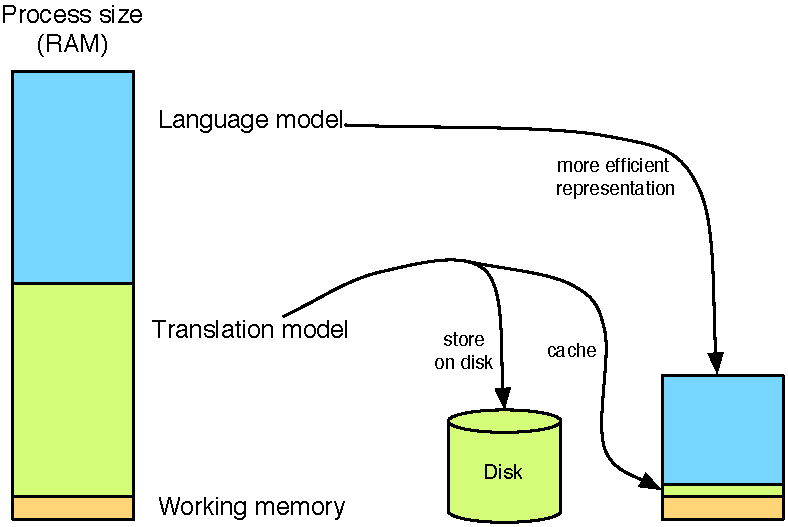
\includegraphics[scale=1.4]{less-memory.pdf}
%\end{center}

%%%%%%%%%%%%%%%%%%%%%%%%%%%%%%%%%%%%%%%%%%%%%%%%%%%%%%%%%%%%%%%%%%%%%%%%%%%%

\slide{Speed vs. Memory Use}
\begin{tabular}{p{10cm}c}
\vspace{-11cm}
Typical Europarl file sizes:
\begin{itemize} \itemsep -1mm
  \item Language model \vspace{-3mm}
	\begin{itemize}
  	\item  170 MB (trigram)
	\item 412 MB (5-gram)
	\end{itemize}
  \item Phrase table \vspace{-3mm}
	\begin{itemize}
  	\item  11GB
	\end{itemize}
  \item Lexicalized reordering \vspace{-3mm}
	\begin{itemize}
  	\item  9.4GB
	\end{itemize}
   \item[$\rightarrow$] total = 20.8 GB
\end{itemize}
&
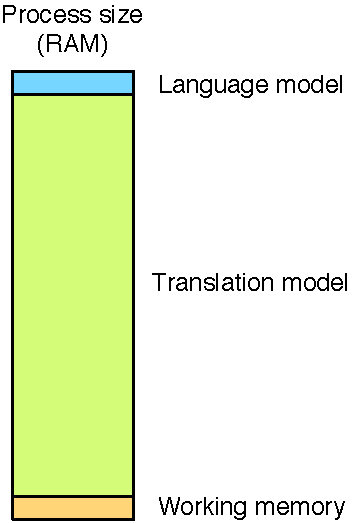
\includegraphics[scale=1.4]{less-memory-europarl.pdf}
\end{tabular}


%%%%%%%%%%%%%%%%%%%%%%%%%%%%%%%%%%%%%%%%%%%%%%%%%%%%%%%%%%%%%%%%%%%%%%%%%%%%

\slide{Binary Phrase Tables}
Create:
\begin{center}
\begin{SaveVerbatim}{myverb} 
  ./CreateOnDiskPt 1 1 4 100 2 pt.txt out.folder
\end{SaveVerbatim}
\colorbox{gray}{\BUseVerbatim{myverb}}
\end{center}

Change ini file: \\[-6mm]
\begin{center}
\begin{SaveVerbatim}{myverb} 
[feature]
PhraseDictionaryOnDisk name=TranslationModel0 \
   table-limit=20 \ num-features=4 \
   path=/.../phrase-table
\end{SaveVerbatim}
\colorbox{gray}{\BUseVerbatim{myverb}}
\end{center}

Notes:
\begin{itemize} \itemsep -1mm
  \item Prune target phrases
  \item Does not sort by weighted score
\end{itemize}

%%%%%%%%%%%%%%%%%%%%%%%%%%%%%%%%%%%%%%%%%%%%%%%%%%%%%%%%%%%%%%%%%%%%%%%%%%%%

\slide{Create Binary Tables}
Create:  
\begin{center}
\small
\begin{SaveVerbatim}{myverb} 
  export LC_ALL=C 
  cat pt.txt | sort | ./processPhraseTable -ttable 0 0 -  \
      -nscores 4 -out out.file
\end{SaveVerbatim}
\colorbox{gray}{\BUseVerbatim{myverb}}

\end{center}

Change ini file: \\[-6mm]
\begin{center}
\begin{SaveVerbatim}{myverb} 
[feature]
PhraseDictionaryBinary name=TranslationModel0 \
   table-limit=20 \ num-features=4 \
   path=/.../phrase-table
\end{SaveVerbatim}
\colorbox{gray}{\BUseVerbatim{myverb}}
\end{center}

Notes:
\begin{itemize} \itemsep -1mm
  \item Does not support hierarchical model
\end{itemize}

%%%%%%%%%%%%%%%%%%%%%%%%%%%%%%%%%%%%%%%%%%%%%%%%%%%%%%%%%%%%%%%%%%%%%%%%%%%%

\slide{Compact Phrase Table}
\begin{itemize}
\item Memory-efficient data structure
\begin{itemize}
\item phrase table 6--7 times smaller than on-disk binary table
\item lexical reordering table 12--15 times smaller than on-disk binary table
\item Fastest phrase-table implementation
\end{itemize}
\item Create with
\begin{center}
\begin{SaveVerbatim}{myverb} 
processPhraseTableMin
processLexicalTableMin
\end{SaveVerbatim}
\colorbox{gray}{\BUseVerbatim{myverb}}
\end{center}
\item Change moses.ini file to use
\begin{center}
\begin{SaveVerbatim}{myverb} 
PhraseDictionaryCompact
\end{SaveVerbatim}
\colorbox{gray}{\BUseVerbatim{myverb}}
\end{center}
\end{itemize}

%%%%%%%%%%%%%%%%%%%%%%%%%%%%%%%%%%%%%%%%%%%%%%%%%%%%%%%%%%%%%%%%%%%%%%%%%%%%

\includepdf[pages={1-47}]{compact-pt.pdf}

%%%%%%%%%%%%%%%%%%%%%%%%%%%%%%%%%%%%%%%%%%%%%%%%%%%%%%%%%%%%%%%%%%%%%%%%%%%%
\slide{Suffix-Array Phrase-table}

\small
\begin{itemize}
  \item stores word-aligned parallel corpus
  \item smaller than phrase-table
  \item Dynamic
    \begin{itemize}
    \item Add more data during decoding
    \item incremental training
    \end{itemize}
  \item Phrase-base only (for the moment)
\end{itemize}

\item Change moses.ini file to use
\begin{center}
\begin{SaveVerbatim}{myverb} 
PhraseDictionaryBitextSampling name=PT0 \
        num-features=9 path=/some/path/${CORPUS} L1=${L1} L2=${L2}
\end{SaveVerbatim}
\colorbox{gray}{\BUseVerbatim{myverb}}

%%%%%%%%%%%%%%%%%%%%%%%%%%%%%%%%%%%%%%%%%%%%%%%%%%%%%%%%%%%%%%%%%%%%%%%%%%%%

\slide{KENLM}
\vspace{10mm}
\begin{itemize}
\item Developed by Kenneth Heafield (CMU / Edinburgh / Stanford / Bloomberg)
\item Fastest and smallest language model implementation
\item Create binary LM from text ARPA LM\\[5mm]
\begin{SaveVerbatim}{myverb} 
build_binary model.lm model.binlm
\end{SaveVerbatim}
\colorbox{gray}{\BUseVerbatim{myverb}}
\item Specify in decoder\\[5mm]
\begin{SaveVerbatim}{myverb} 
[feature]
KENLM name=LM0 factor=0 path=/.../model.binlm order=5
\end{SaveVerbatim}
\colorbox{gray}{\BUseVerbatim{myverb}}
\end{itemize}

%%%%%%%%%%%%%%%%%%%%%%%%%%%%%%%%%%%%%%%%%%%%%%%%%%%%%%%%%%%%%%%%%%%%%%%%%%%%

\slide{KENLM}

Three language models in 1
\begin{itemize}
\item Probing
  \begin{itemize}
  \item Fast
  \item Uses hash table
  \end{itemize}
\item Trie
  \begin{itemize}
  \item Small
  \item Uses sorted arrays
  \end{itemize}
\item Chop
  \begin{itemize}
  \item Smaller
  \item Trie with compressed pointers
  \end{itemize}
\end{itemize}

%%%%%%%%%%%%%%%%%%%%%%%%%%%%%%%%%%%%%%%%%%%%%%%%%%%%%%%%%%%%%%%%%%%%%%%%%%%%

\slide{DALM (Double Array Language Model)}

\begin{center} 
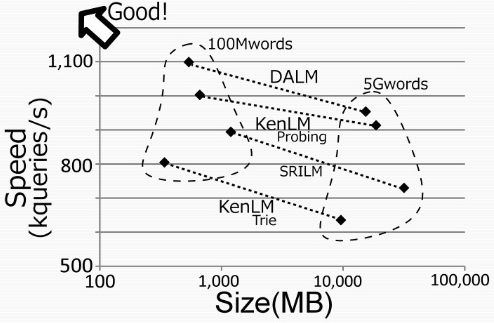
\includegraphics[scale=1.0]{DALM.png}\vspace{-20mm}
\end{center}

%%%%%%%%%%%%%%%%%%%%%%%%%%%%%%%%%%%%%%%%%%%%%%%%%%%%%%%%%%%%%%%%%%%%%%%%%%%%

\slide{Decoding paradigms/algorithms}

Multiple algorithms
\begin{itemize}
  \item Phrase-models
    \begin{itemize}
    \item Standard
    \item Cube-Pruning
    \end{itemize}
  \item Synchronous CFG
    \begin{itemize}
    \item Cube-Pruning
    \item Scope-3
    \item incremental (Ken's)
    \end{itemize}
  \item Synchronous TSG
  
\end{itemize}

%%%%%%%%%%%%%%%%%%%%%%%%%%%%%%%%%%%%%%%%%%%%%%%%%%%%%%%%%%%%%%%%%%%%%%%%%%%%

\includepdf[pages={1-13}]{Sennrich_Ssst2014_slides.pdf}


\end{document}

